\documentclass[xcolor=svgnames,11pt]{beamer}

\usepackage{graphicx}

\usepackage[italian, english]{babel} 
\usepackage[utf8x]{inputenc}

\usepackage{hyperref}
\usepackage{tabularx}
\usepackage{url}

\usetheme{Goettingen}
\definecolor{raspi}{HTML}{bb1142}
\definecolor{green_raspi}{HTML}{75aa28}
\definecolor{myblack}{RGB}{34,34,34}

\usecolortheme[named=green_raspi]{structure}

\beamertemplateshadingbackground{white!15}{raspi!5}
\setbeamertemplate{sidebar canvas right}[vertical shading]%
[top=raspi!50,bottom=white!90]

\setbeamertemplate{blocks}[rounded][shadow=false]
\setbeamercolor{block body}{bg=green_raspi!30}
\setbeamercolor{block title}{bg=green_raspi!90}

\setbeamercovered{transparent}

\title{\textbf{Raspberry Pi - Il computer che hai sempre voluto avere}}
\author{Nicola Corti}
\institute{Linux Day 2014 - Pisa \\ \medskip 
\includegraphics[height=1.5cm]{ld_logo.png} \hspace{1cm} 
\includegraphics[height=1.5cm]{gulp_logo.png}}
\logo{gulp_logo.png}
\date{26 ottobre 2014}

 
\begin{document}

\begin{frame}
	\titlepage
\end{frame}

\section{Introduzione}

\begin{frame}{Cosa \`e il Raspberry Pi}
\begin{center}
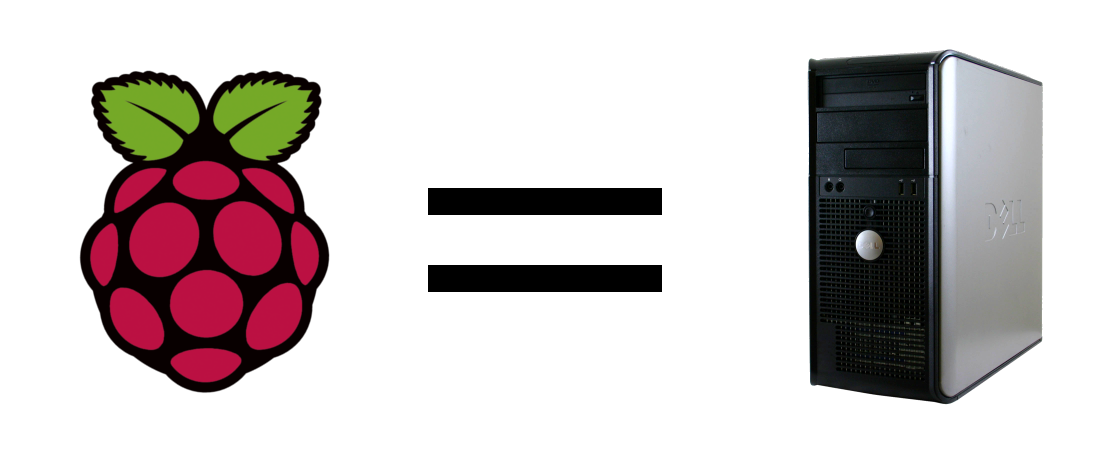
\includegraphics[width=9cm]{isapc.png}
\end{center}
\end{frame}

\begin{frame}{Cosa \`e il Raspberry Pi}

\pause

Il Raspberry Pi \`e a tutti gli effetti un \textbf{computer}, che ci permette sostanzialmente di effettuare le stesse operazioni che faremo con un computer classico.

\pause

\begin{block}{Cosa \`e?}
\emph{
Il Raspberry Pi è un single-board computer (un calcolatore implementato su una sola scheda elettronica).}
\begin{flushright}
\begin{footnotesize}
\emph{Da Wikipedia, l'enciclopedia libera.}
\end{footnotesize}
\end{flushright}

\end{block}

\pause
\medskip

...per\`o \`e pi\`u \textbf{piccolo}!

\end{frame}

\begin{frame}{Cosa \`e il Raspberry Pi}
\begin{center}
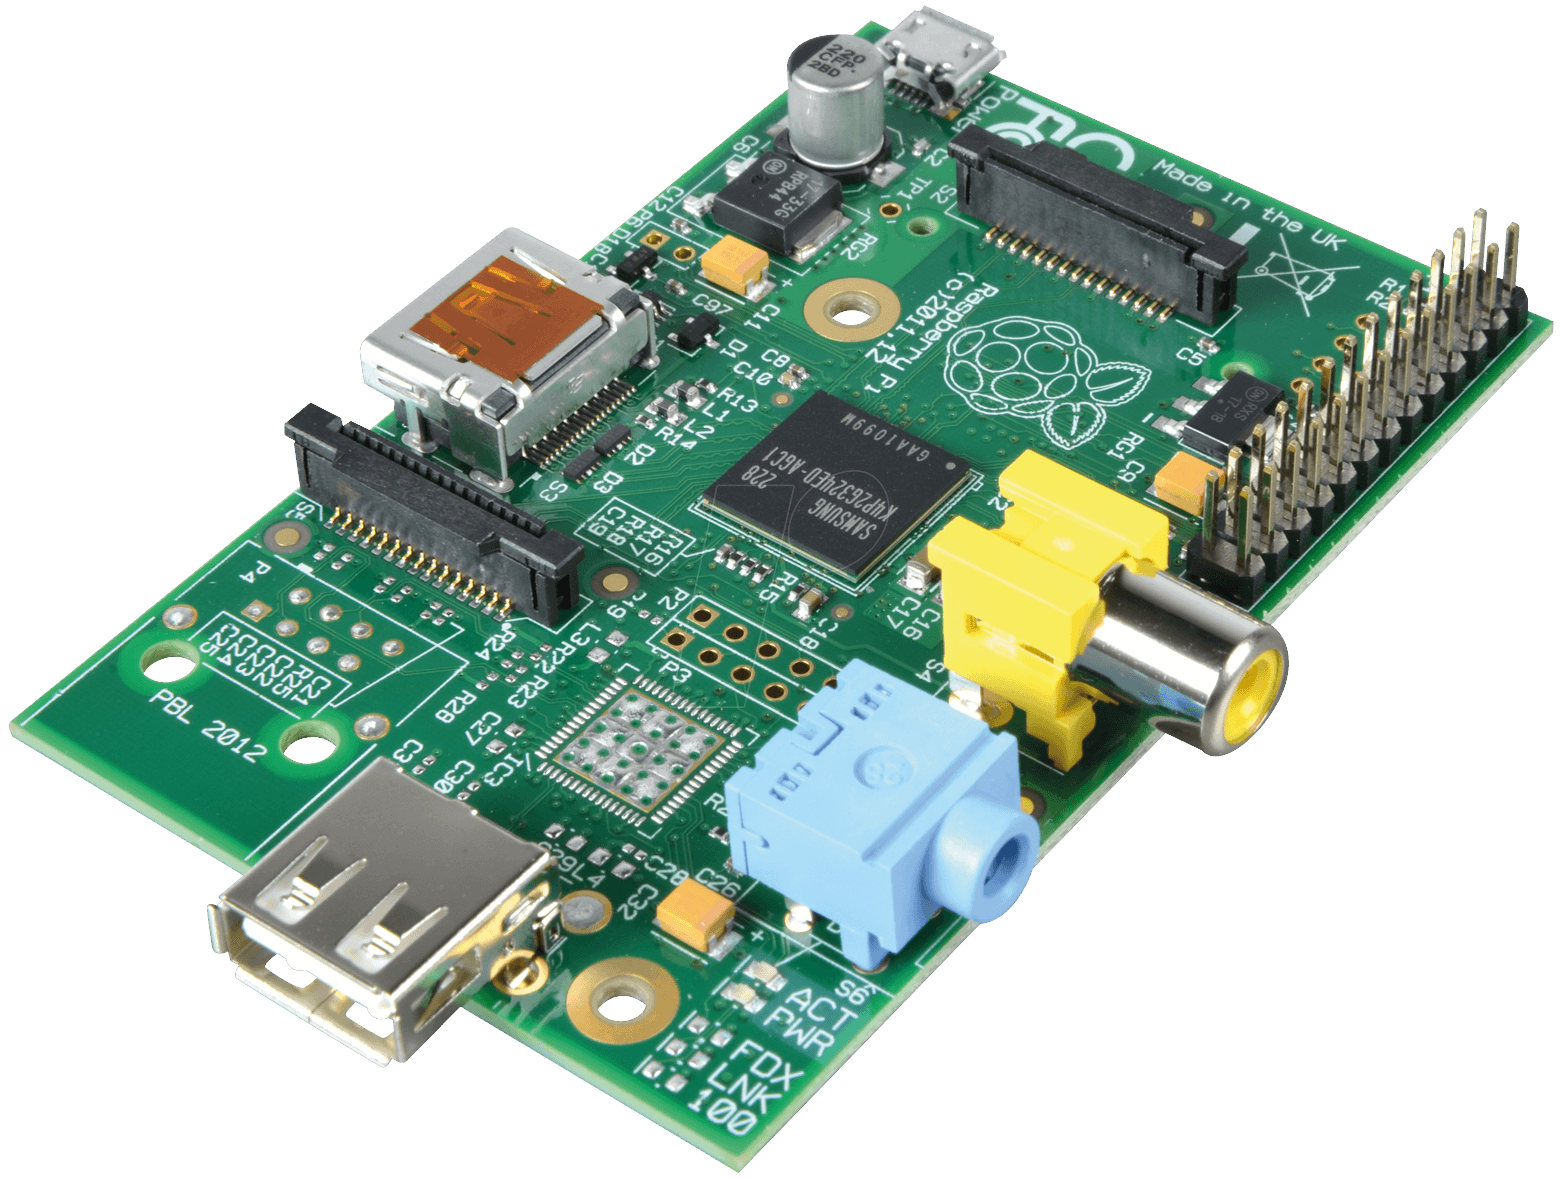
\includegraphics[width=9cm]{raspi.png}
\end{center}
\end{frame}


\begin{frame}{Come nasce il Raspberry Pi}
\begin{center}

\includegraphics[width=6cm]{logo_raspi.png}
\end{center}
\pause

Il Raspberry Pi nasce nel Regno Unito, realizzato dalla \emph{Raspberry Pi Foundation}

\begin{center}
\url{http://www.raspberrypi.org/}
\end{center}

\pause
\medskip

\`E nato con l'intendo di creare un computer:
\pause
\begin{itemize}
\item Per avvicinare alla programmazione,
\pause
\item Per la didattica nelle scuole,
\pause
\item Che sia economicamente accessibile.
\end{itemize}
\end{frame}

\begin{frame}{Raspberry Pi - Model B}
\begin{center}
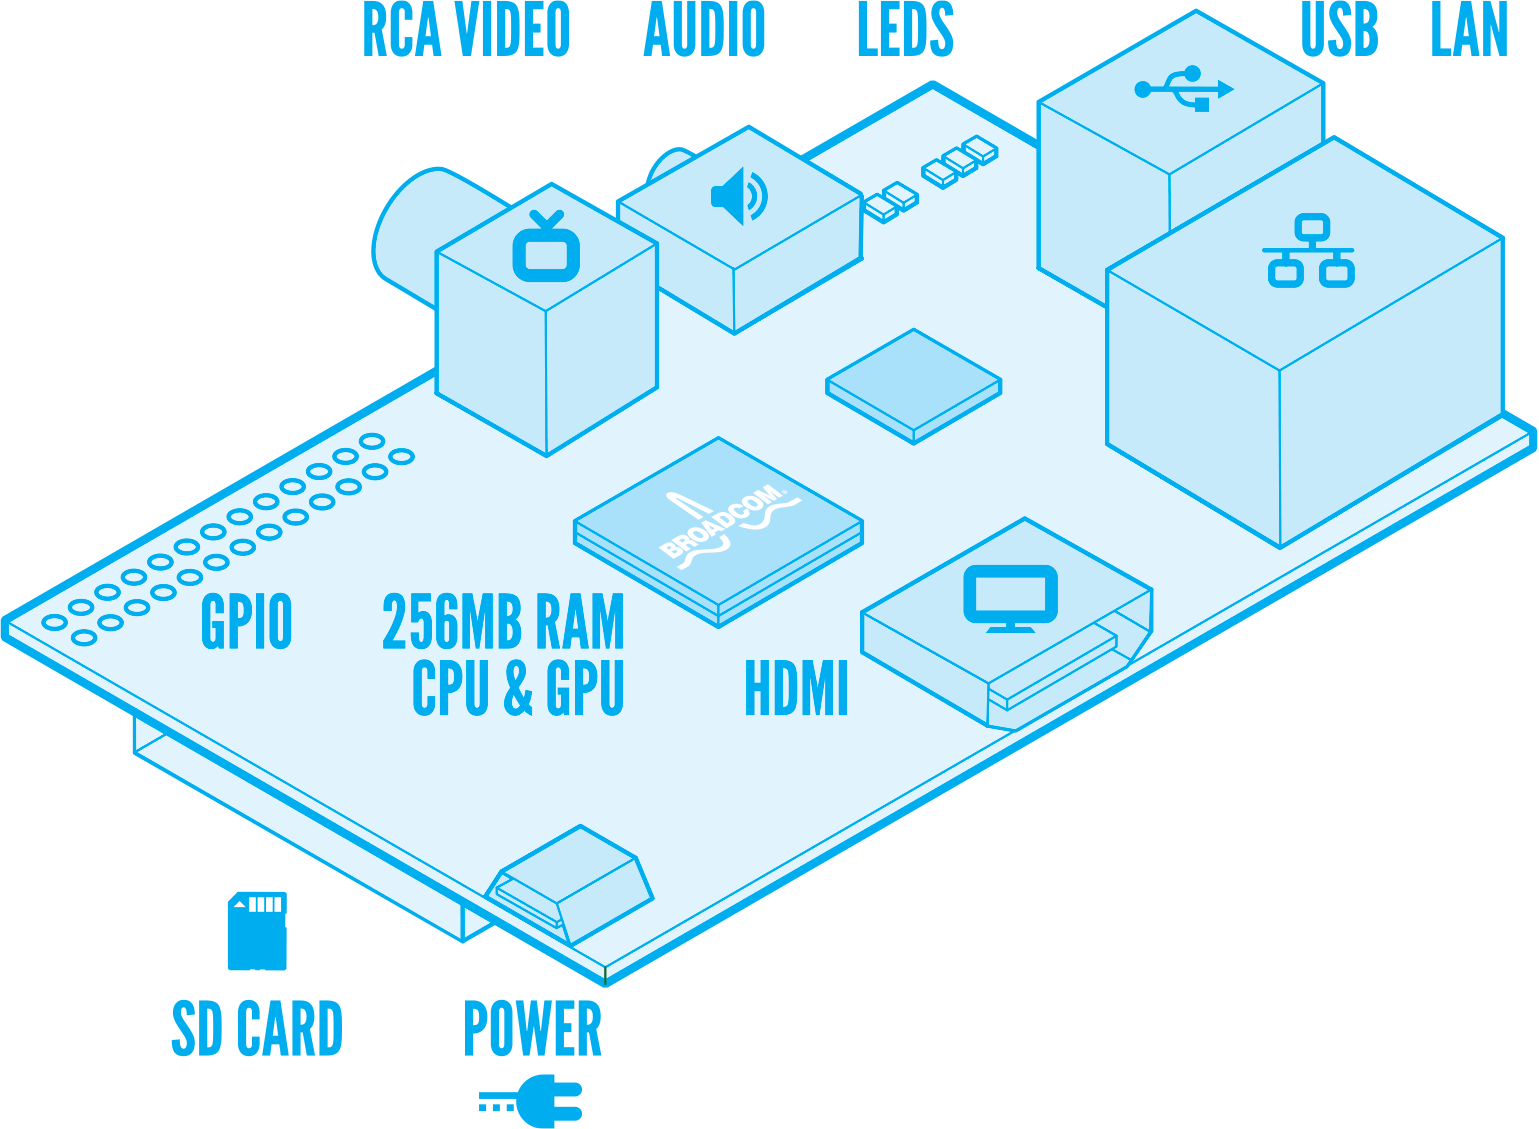
\includegraphics[width=9cm]{scheme.png}
\end{center}
\end{frame}

\begin{frame}{Quali modelli di Raspberry Pi}
\begin{center}
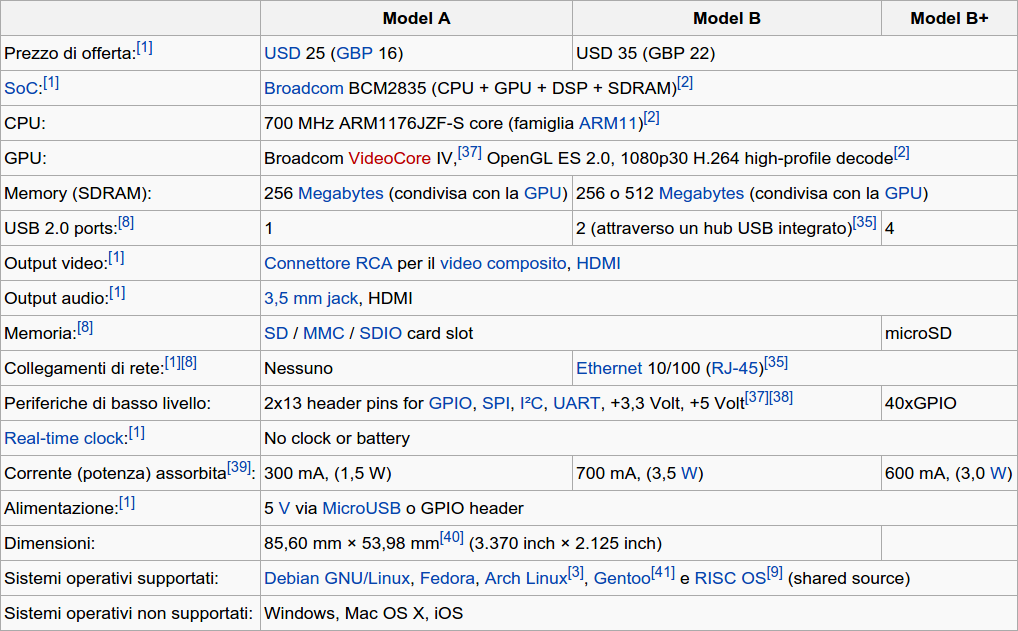
\includegraphics[width=9.5cm]{table.png}
\end{center}
\end{frame}

\begin{frame}{Cosa serve per far funzionare un Raspberry Pi}
Per iniziare a divertirci con il nostro Raspberry Pi avremo bisogno di:
\pause
\begin{description}
\item[Alimentatore] Micro USB, Output a 1200 $mA$.
\pause
\item[Scheda SD] Da almeno 2 GB, meglio se da 4 GB (e possibilmente di classe 10).
\pause
\item[Rete] Connessione ethernet ad internet.
\pause
\item[Input] Mouse e tastiera USB (consigliati).
\pause
\item[Monitor] Con interfaccia HDMI o DVI (consigliati), oppure un televisore con entrata RCA.
\end{description}
\end{frame}

\begin{frame}[fragile]{Accessori per il Raspberry Pi}
Estendiamo il nostro Raspberry Pi tramite:
\vspace{1cm}

\begin{columns}
    \begin{column}{0.5\textwidth}
	\begin{itemize}
	\item Pi-Camera
	\pause
	\item Touch Screen LCD
	\pause
	\item Hub USB
	\pause
	\item Dongle Wifi (Bluetooth o 3G)
	\pause
	\item Case
	\end{itemize}
    \end{column}
    \begin{column}{0.5\textwidth}
    \begin{center}
      \includegraphics<1>[height=4cm]{picamera.png}
      \includegraphics<2>[height=4cm]{pimonitor.png}
      \includegraphics<3>[height=4cm]{pihub.png}
      \includegraphics<4>[height=4cm]{piwifi.png}
      \includegraphics<5>[height=4cm]{picase.png}            
    \end{center}
    \end{column}
  \end{columns}
\end{frame}

\begin{frame}{Dove comprare il Raspberry Pi}

\begin{center}

\includegraphics[width=5cm]{wherebuy.png}
\end{center}

\`E possibile acquistare il Raspberry Pi presso uno dei distributori ufficiali, oppure anche su qualsiasi altro shop online che venda articoli di elettronica.

\medskip

Il costo per i modelli B/B+ si aggira intorno ai \textbf{35 euro}.

\end{frame}

\section{Distribuzioni Linux}

\begin{frame}{Raspbian}
\begin{center}

\includegraphics[width=6cm]{raspbian_logo.png}
\end{center}

\pause
\medskip

\textbf{Raspbian} \`e una versione modificata di \emph{Debian Wheezy} (una delle pi\`u famose distribuzioni di Linux) ottimizzata per architettura \textbf{arm}.

\pause
\medskip

Raspbian fornisce un insieme molto grande di pacchetti gi\`a funzionanti per Raspberry Pi, installabili tramite il famoso comando \texttt{apt-get install}.

\pause
\medskip
\begin{center}
\url{http://www.raspbian.org/}
\end{center}
\end{frame}

\begin{frame}[fragile]{Raspbmc - OpenELEC}

\begin{columns}
    \begin{column}{0.5\textwidth}
    \begin{center}
    
    
\includegraphics[height=2cm]{raspbmc_logo.png}

    \end{center}	
	\end{column}

    \begin{column}{0.5\textwidth}
    \begin{center}
    
    
\includegraphics[height=2cm]{open_elec.png}

    \end{center}	
	\end{column}
\end{columns}

\bigskip
\pause

\textbf{Raspbmc} ed \textbf{OpenELEC} sono due distribuzioni che 	forniscono il media center \textbf{XBMC}, che permette di trasformare il vostro Raspberry Pi in un media center domestico.

\pause
\medskip

Il chip grafico del Raspberry Pi permette di fare il decoding di filmati in formato \textbf{H.264} fino a \textbf{1080p}.

\pause
\begin{center}
\url{http://www.raspbmc.com/} \\
\url{http://openelec.tv/}
\end{center}

\end{frame}

\section{Use cases}

\begin{frame}{}
\begin{center}
\begin{Huge}
Use Cases
\end{Huge}
\end{center}

\end{frame}

\begin{frame}{Media Center}
\begin{center}
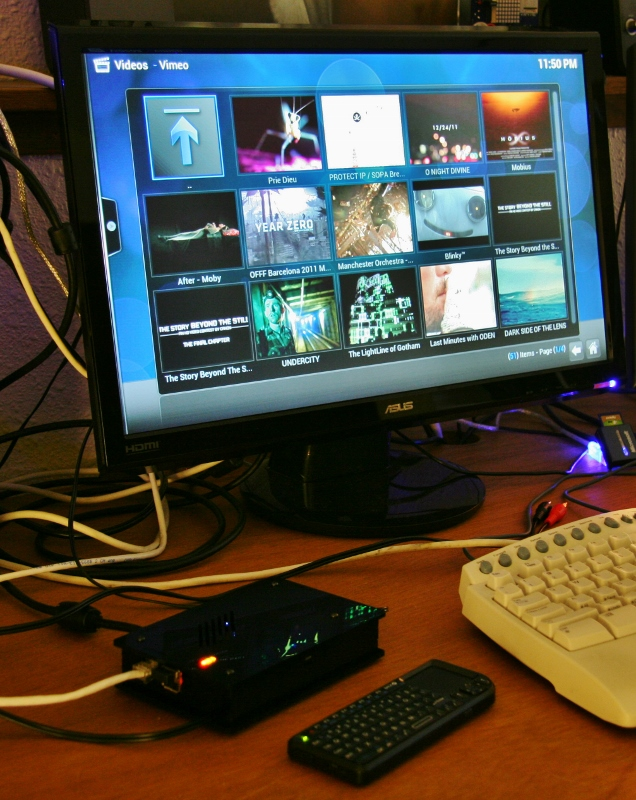
\includegraphics[height=7cm]{uc/media.jpg}
\end{center}
\end{frame}

\begin{frame}{Computer Domestico}
\begin{center}
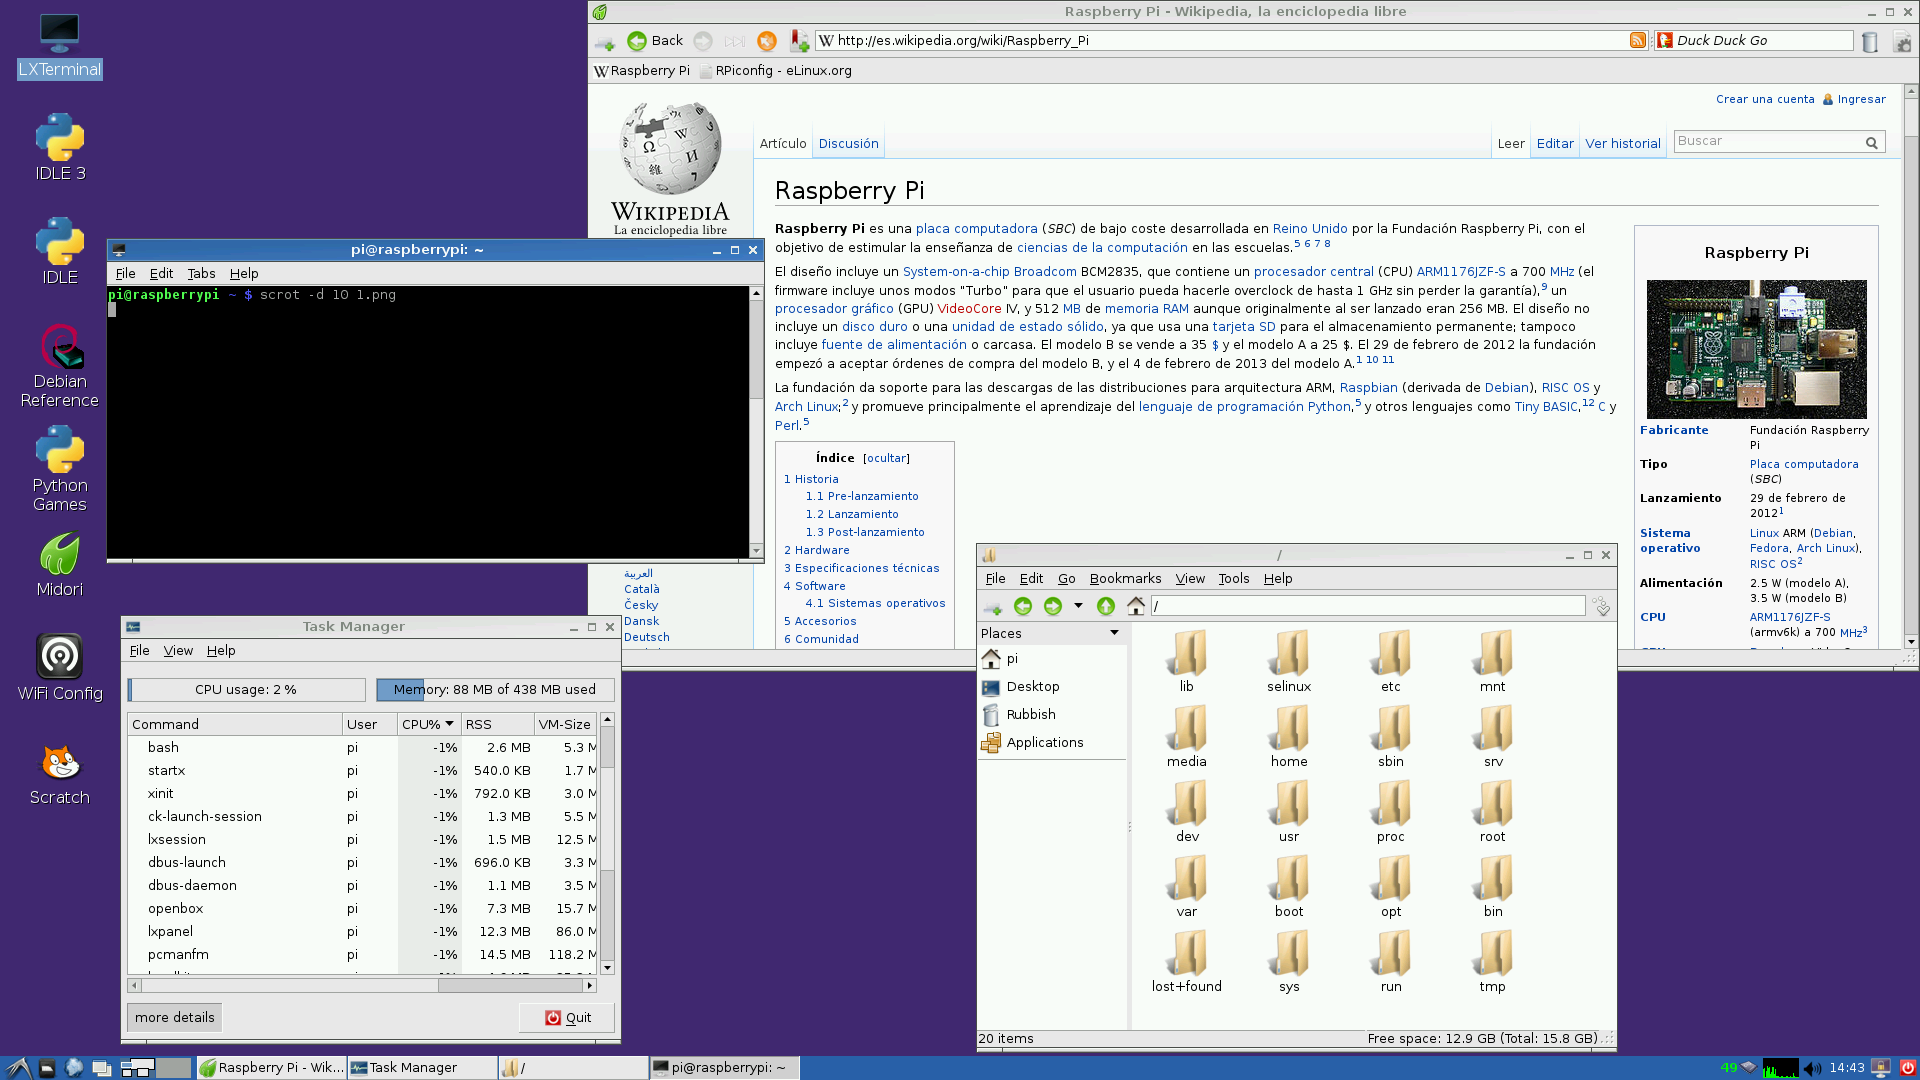
\includegraphics[width=9cm]{uc/pc.png}
\end{center}
\end{frame}

\begin{frame}{Torrent Server}
\begin{center}
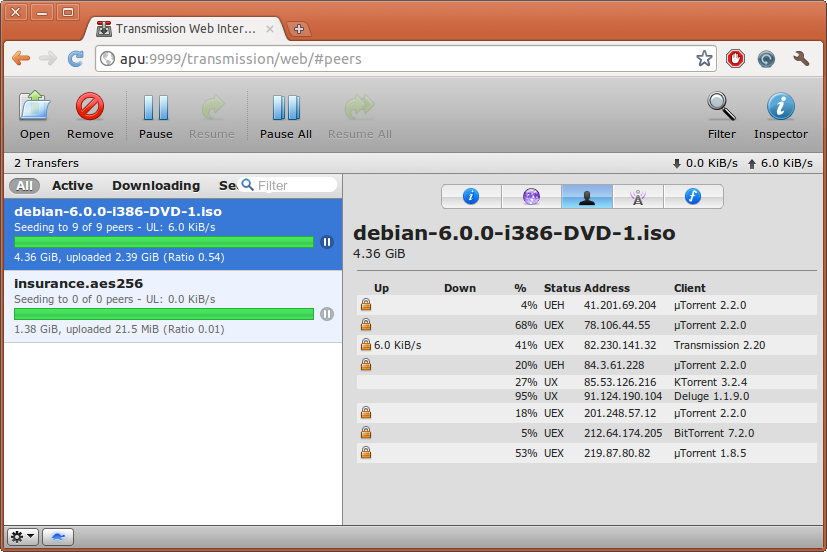
\includegraphics[width=9cm]{uc/torrent.png}
\end{center}
\end{frame}

\begin{frame}{Home security}
\begin{center}
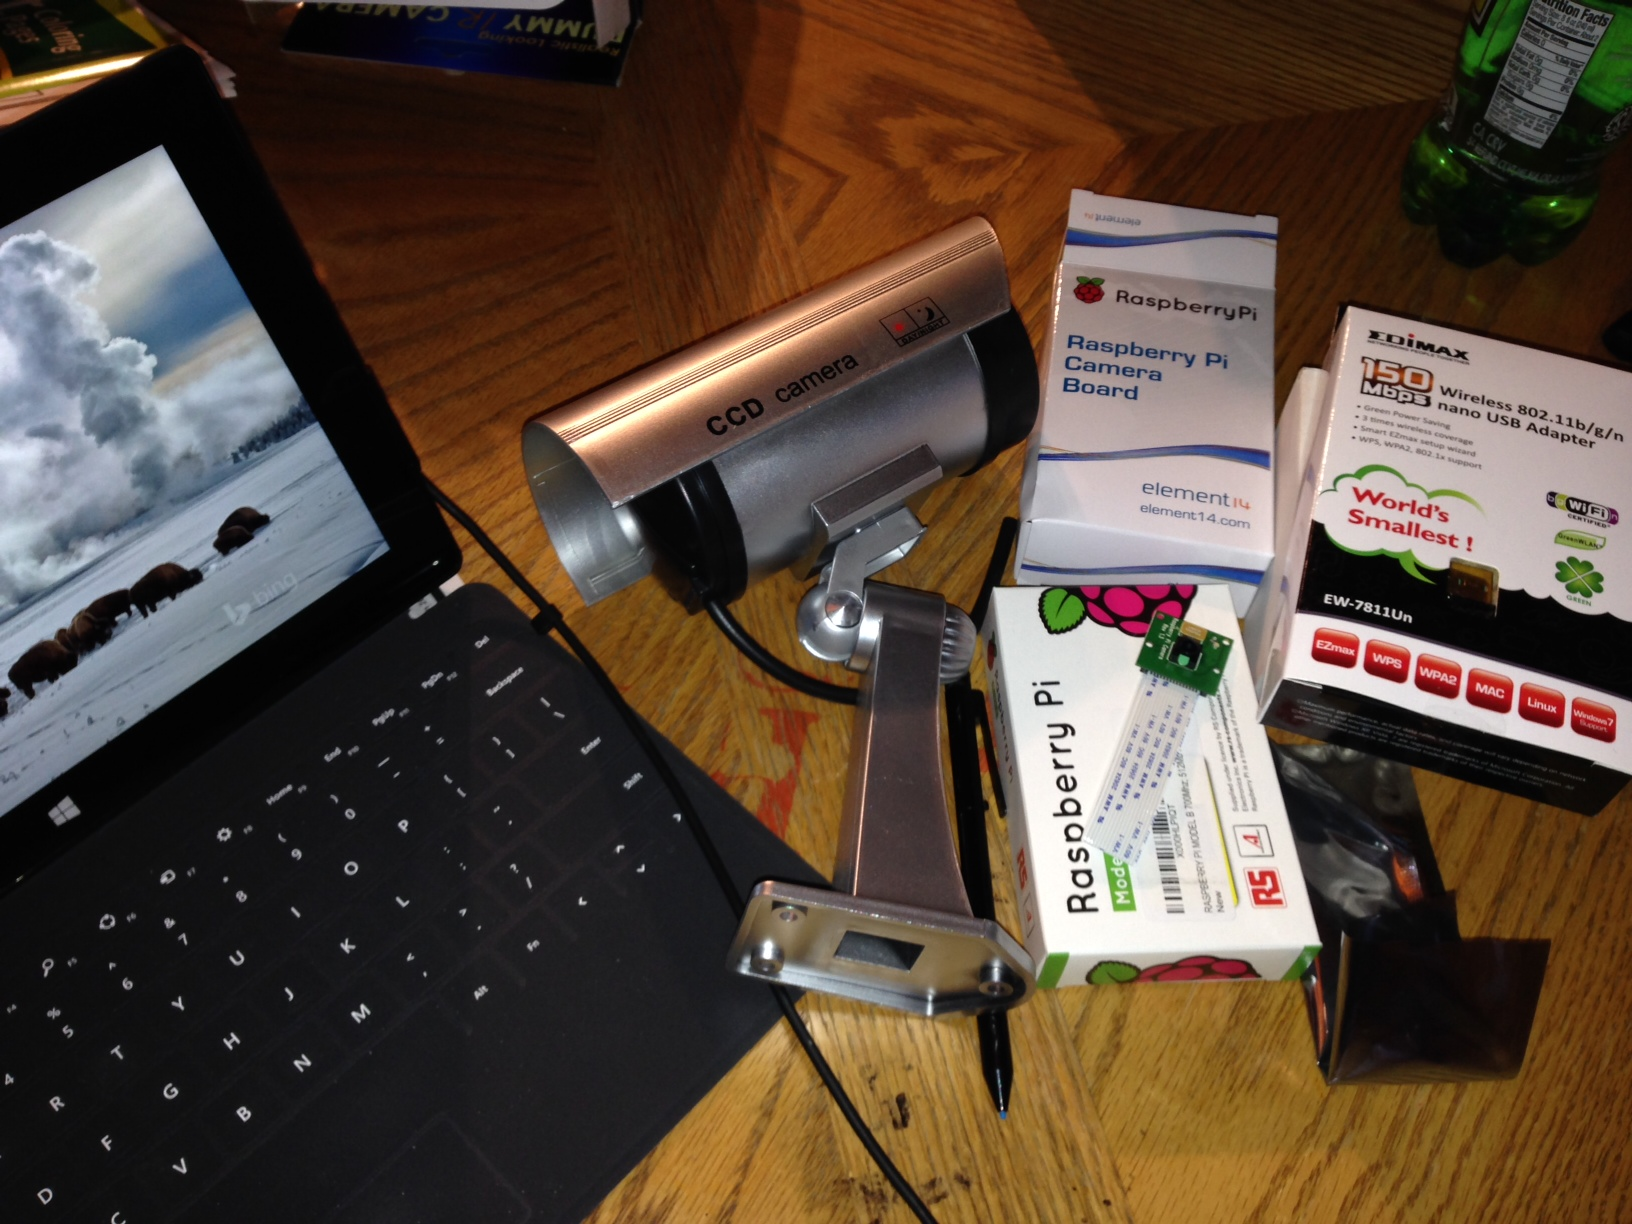
\includegraphics[width=9cm]{uc/security.jpg}
\end{center}
\end{frame}

\begin{frame}{Scratch}
\begin{center}
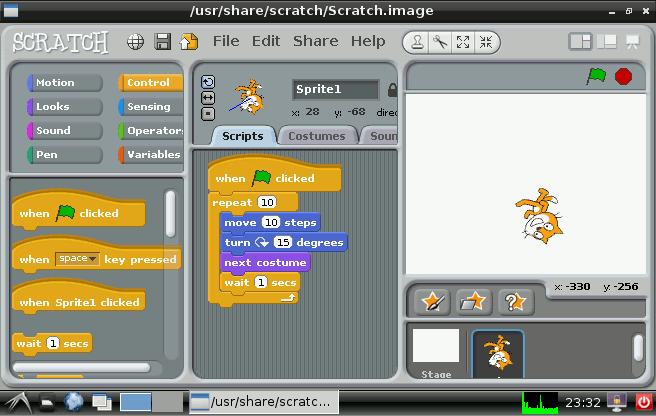
\includegraphics[width=9cm]{uc/scratch.png}
\end{center}
\end{frame}

\begin{frame}{Altro...}
\begin{center}
\includegraphics<1>[width=9cm]{uc/cluster.jpg}
\includegraphics<2>[width=9cm]{uc/arcade.jpg}
\includegraphics<3>[width=9cm]{uc/keyboard.jpg}
\includegraphics<4>[width=9cm]{uc/drone.jpg}

\end{center}
\end{frame}

\section{Prima installazione}

\begin{frame}{}
\begin{center}
\begin{Huge}
Prima installazione
\end{Huge}
\end{center}

\begin{frame}{Prima installazione}
\end{frame}

\begin{frame}{1) Scaricare NOOBS}
\end{frame}

\begin{frame}{2) Formattare la scheda SD}
\end{frame}

\begin{frame}{3) Copiare NOOBS su scheda SD} 
\end{frame}

\begin{frame}{4) Avviare il Raspberry Pi}
\end{frame}

\begin{frame}{5) Scegliere i S.O.}
\end{frame}

\begin{frame}{6) Attendere...}
\end{frame}

\end{document}
